\section{Muons and Lorentz Transformations}

\instructornote{%
By Matt Trawick, 2019.  Time: ?

I could add a bit to clarify the difference between proper distance and proper length.
}

\makelabheader %(Space for student name, etc., defined in master.tex or labmanual_formatting_commands.tex)

\bigskip
\textbf{Apparatus:}
\begin{itemize}[nosep]
\item \textit{Mathematica}, with notebook file \filename{minkowski\_events.nb}
\end{itemize}


\bigskip
\textbf{Activity 1: Muon Lifetime} 


Muons are rare subatomic particles which are not usually found in ordinary matter on Earth.  Muons can be created when protons or atomic nuclei, traveling at high speeds from the sun or other stars, strike the Earth's upper atmosphere and collide with molecules in the air.  As a result of these collisions, there are always muons raining down from the upper atmosphere towards the Earth's surface.

But muons don't last long.  At rest in a laboratory, muons have an average lifetime of only 2.2~$\mu$s, spontaneously decaying into (usually) an electron and two neutrinos.  Given an initial number of muons $N_0$ at time $t=0$, the number of muons $N$ at any later time $t$ is given by
\begin{equation}
N=N_0 e^{-t/\tau},
\end{equation}
where $\tau = 2.2~\mu$s is the muons' average lifetime.  


\begin{enumerate}[labparts]
\item   
Suppose that muons are created in the Earth's atmosphere at a height of 4~km above the surface.  The muons stream towards the ground at a speed of $0.93c$.
How long does it take these muons to reach the surface of the Earth?
\answerspace{0.8in}

\item What fraction of the original muons should be remaining after this time, according to Equation (1)? 
\answerspace{0.6in}

\item The time $\Delta t$ that you calculated in (a) is the time between two specific events: the muon being created and the muon hitting the Earth's surface.  What reference frame measures the \textit{proper time} $\Delta t_0$ between these two events?  Is it the reference frame of a scientist on Earth, or the reference frame of the muon?
\answerspace{0.4in}

\item What is the time of the journey from the upper atmosphere to the ground in the reference frame of the muon, travelling at speed $0.93c$?
\answerspace{0.8in}

\item What fraction of the original muons should be remaining after this time $\Delta t_0$, in the reference frame of the muons?
\answerspace{0.6in}

\item Whatever causes a muon to decay takes place entirely within the muon itself.  (That's why it's called ``spontaneous'' decay; it's not caused by anything external to the muon.)  
Is the time $t$ that governs the average lifetime of a muon the time as measured in the Earth's reference frame, or the muon's reference frame?  
\answerspace{0.4in}

\item If you measure the fraction of muons that \textit{actually} reach the ground, what fraction will you observe?
(This observation was first done in the 1920s, and was an early experimental confirmation of Einstein's theory of relativity.)
\answerspace{0.4in}

\item One more thing.  In part (d), you probably calculated the muons' $\Delta t_0$ using the idea of time dilation.  Now, try doing it again using the idea of length contraction.  In the reference frame of the muon, what is the distance between the upper atmosphere and the ground?
\answerspace{0.8in}

\item How long does it take the muon to travel that distance?
\answerspace{0.6in}

\end{enumerate}

\begin{wrapfigure}[8]{r}{0.35\textwidth}
\begin{center}
%\vspace{-0.3in}
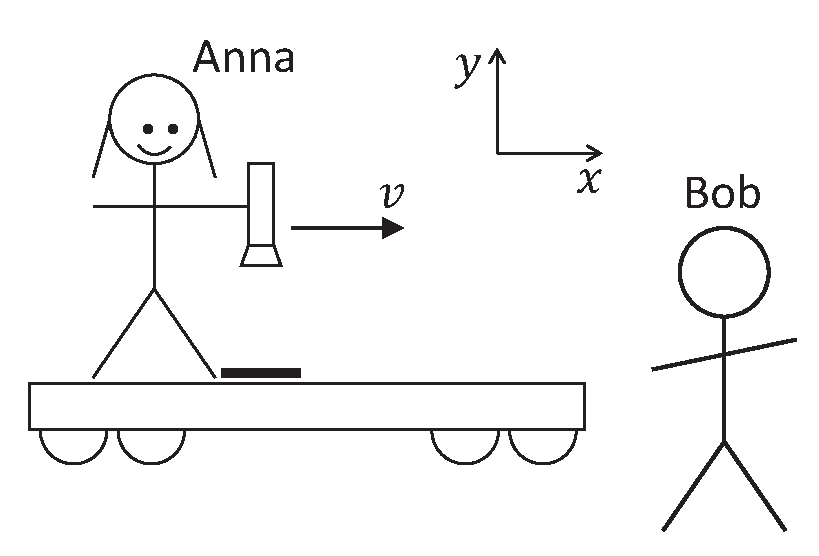
\includegraphics[scale=0.4]{../../205/labmanual/time_dilation_length_contraction/anna_and_bob.eps}
\end{center}
\end{wrapfigure}


\textbf{Activity 2: Lorentz Transformations}


\begin{enumerate}[labparts]

\item  
You have previously discussed a thought experiment in which Anna rides a train at speed $v$.  She aims a laser beam at a mirror on the floor of the train, and measures the time $\Delta t_0$ that it takes from the time the photon is emitted to when the photon returns to the laser.  Bob observes the same experiment, standing near the tracks beside the train.  On the axes below on the left, draw a spacetime graph (Minkowski diagram) of these two events as seen in Anna's reference frame, taking the emission of the photon to happen at $x=0$ and $t=0$.
\end{enumerate}

\begin{center}
\raisebox{0.7in}{Galilean Transformation:}\hspace{0.2in}
\begin{lab_axis}[lab_noticks_4quads,
	width=1.5in, height=1.5in,
	xlabel={$x$},
	ylabel={$t$},
	title={Anna's Frame}
	]
\end{lab_axis}
\hspace{0.3in}
\begin{lab_axis}[lab_noticks_4quads,
	width=1.5in, height=1.5in,
	xlabel={$x$},
	ylabel={$t$},
	title={Bob's Frame}
	]
\end{lab_axis}
\end{center}
\begin{enumerate}[labparts,resume]

\item 
Now consider the same two events in the reference frame of Bob.  
On the axes above on the right, draw a spacetime graph of these two events as seen in Bob's reference frame, according to the principle of Galilean relativity (as described the Galilean transformations).

\item Once you have drawn your graph, you can check your answer by 
opening the file \filename{minkowski\_events.nb}, which will open in Mathematica.  Type \button{Ctrl-A} to select everything, and type \button{Shift-Enter} to excute all of the lines you have selected.  Then scroll down to the first graph you see, titled ``Galilean Transformation''.  You will need to edit the line that graphs the two green points.  Make any corrections needed on your graphs above.

\item The graph you drew for Bob's reference frame is inconsistent with the principle of relativity, because it implies that the speed of light is not the same in all reference frames.  In Anna's frame, light travels only the vertical distance down and back in some time $t$.  In Bob's frame, the light travels a longer, diagonal path.  According to the Galilean transformations, it does so in the same time $t$ as in Anna's frame, which would mean that Bob would see the light going faster than Anna does.  To correct this, would the time $t$ of the light returning to the flashlight be \textit{earlier} or \textit{later} than in Anna's frame?
\answerspace{0.4in}

\item On the axes below, redraw the two events as seen in Anna's reference frame on the axes to the left.  On the axes on the right, draw the two events as you know they should be, consistent with the principle of relativity.

\begin{center}
\raisebox{0.7in}{Lorentz Transformation:}\hspace{0.2in}
\begin{lab_axis}[lab_noticks_4quads,
	width=1.5in, height=1.5in,
	xlabel={$x$},
	ylabel={$t$},
	title={Anna's Frame}
	]
\end{lab_axis}
\hspace{0.3in}
\begin{lab_axis}[lab_noticks_4quads,
	width=1.5in, height=1.5in,
	xlabel={$x$},
	ylabel={$t$},
	title={Bob's Frame}
	]
\end{lab_axis}
\end{center}

\item Once you have drawn your graph, you can check your answers again using the same Mathematica simulation as before, but this time scroll down further to the second graph, titled "Lorentz Transformation''.  Again, edit the positions of the two green points, and move the slider to represent the speed of Bob's reference frame relative to Anna's.  Was your prediction correct?  Note any corrections on the graphs above, as needed. 
\end{enumerate}

\textbf{Activity 3: More fun with Anna and Bob}

In class, we imagined an experiment in which Anna held out her arms with a lightbulb in each hand, turning on the lightbulbs simultaneously.  Take each of Anna’s arms to be one meter long.

\begin{enumerate}[labparts]
\item On the axes below on the left, draw a spacetime diagram in the reference frame of Anna showing three events: each of the two lightbulbs turning on, and the photons from both bulbs arriving at the tip of Anna’s nose.  Take the photons arriving at Anna’s nose to happen at $x=0$ and $t=0$.  On the axes to the right, draw the same three events as they would occur in Bob's reference frame, moving to the left with velocity $v=-0.5c$, \textit{according to the Galilean transformations.}

\begin{center}
\raisebox{0.7in}{Galilean Transformation:}\hspace{0.2in}
\begin{lab_axis}[lab_noticks_4quads,
	width=1.5in, height=1.5in,
	xlabel={$x$},
	ylabel={$t$},
	title={Anna's Frame}
	]
\end{lab_axis}
\hspace{0.3in}
\begin{lab_axis}[lab_noticks_4quads,
	width=1.5in, height=1.5in,
	xlabel={$x$},
	ylabel={$t$},
	title={Bob's Frame}
	]
\end{lab_axis}
\end{center}

\item As before, check your results using the \textit{Galilean Transformation} simulation in Mathematica, noting any corrections on your axes above.

\item Are the two graphs above consistent with the principle of relativity?  Why or why not?
\answerspace{0.6in}

\item On the axes below, redraw the same three events in both Anna's reference frame and Bob's reference frame, according to the Lorentz transformation.  You can try it on your own first if you like, then use the Lorentz Transformation simulation in Mathematica to confirm or correct your understanding.

\begin{center}
\raisebox{0.7in}{Lorentz Transformation:}\hspace{0.2in}
\begin{lab_axis}[lab_noticks_4quads,
	width=1.5in, height=1.5in,
	xlabel={$x$},
	ylabel={$t$},
	title={Anna's Frame}
	]
\end{lab_axis}
\hspace{0.3in}
\begin{lab_axis}[lab_noticks_4quads,
	width=1.5in, height=1.5in,
	xlabel={$x$},
	ylabel={$t$},
	title={Bob's Frame}
	]
\end{lab_axis}
\end{center}

\item In the graphs above, is light traveling at speed $c$ in both reference frames?
\answerspace{0.6in}

\item Are the two events of the bulbs turning on simultaneous in both reference frames?


\end{enumerate}
